\chapter[SCP-165 贪婪蠕沙]{
    SCP-165 The Creeping, Hungry Sands of Tule\\
    SCP-165 贪婪蠕沙
}

\label{chap:SCP-165}

\begin{figure}[H]
    \centering
    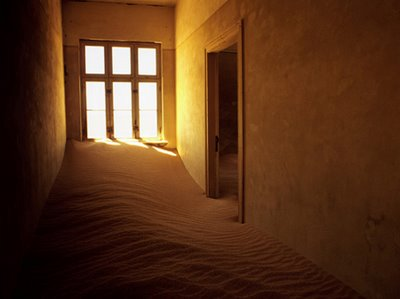
\includegraphics[width=0.5\linewidth]{images/SCP-165.jpg}
    \caption*{在一栋废弃的建筑之中,SCP-165从太阳的热量之中逃离}
\end{figure}

\bb{项目编号:}SCP-165

\bb{项目等级:}Keter

\bb{特殊收容措施:}现收容于一个位于武装生物收容Area-14(Armed Bio-Containment Area-14)中一个设施之中的SCP-165应被认为是一个有传染性的、病态的生物。应对其实施最高的杀菌和检疫手段。

微波场产生器应被放置于SCP-165的收容区域之中的正确位置来限制在它收容区域之中的的沙丘移动,每9天,SCP-165应用不少于750kg的牲畜进行喂养。

\hr

\bb{描述:}SCP-165的有机组分是由典型的寄生虫所构成的,这些寄生虫大约有750μm长,有8条腿并且有着与尘螨相近的基因结构。主要不同的地方就是这种虫子像寄居蟹一样的将沙子往自己身上堆积的习性。现在仍不知道这些沙子作用为何,但是数量庞大的SCP-165族群,可能是数以千亿计到数以万亿计,构成了一个巨大的沙丘。

\begin{figure}[H]
    \centering
    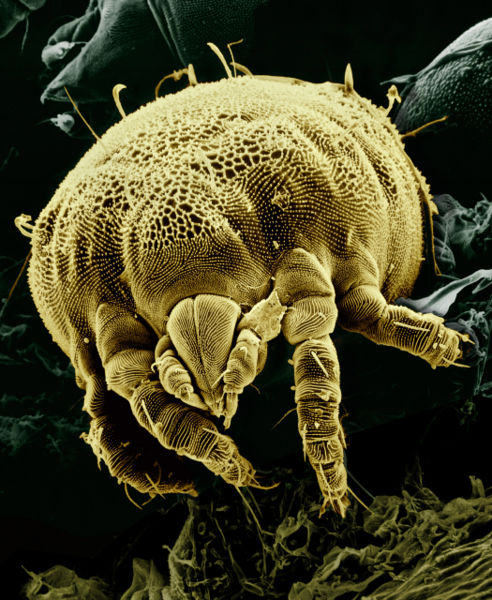
\includegraphics[width=0.5\linewidth]{images/SCP-165-2.jpg}
    \caption*{一张SCP-165的电镜成像}
\end{figure}

在{[}数据删除]和SCP-165之间的共同点只是表面而已,{[}数据删除]的族群是自然界的原生生物并且表现出了一种现在尚不能理解的集群智慧和意识。SCP-165的族群则是由一个个单独的壁虱构成,这些壁虱在捕食时没有表现出合作,而更多的是竞争。像蚊子一样,它们通过对空气之中的二氧化碳和糖分的化学探测来确定猎物的位置。这些 寄生虫会往猎物的方向相互翻滚着、束缚着,仅仅用它们的足来爬过一个又一个的同类。当接触到动物的肉体时,它们将会通过叮咬来释放一种麻痹性的化学毒素,这种毒素非常像蚊子和跳蚤产生的叮咬毒素。项目往往都不知道这些虫子云集在它的身边时,数以百万计的的寄生虫正在“轮流”大口地撕咬着它的血肉。

一种典型的虫群形态是这些寄生虫在猎物或者猎物的肢体附近形成了令人晕眩的漩涡。在SCP-165的环绕竞争之中,这虫群有足够的效率将生物的肢体剥去筋肉,在数分钟之内就只剩白骨。这些麻痹性毒素是如此地有效以至于熟睡的猎物在其肢体被啃食殆尽之后都不会醒来。

\begin{figure}[H]
    \centering
    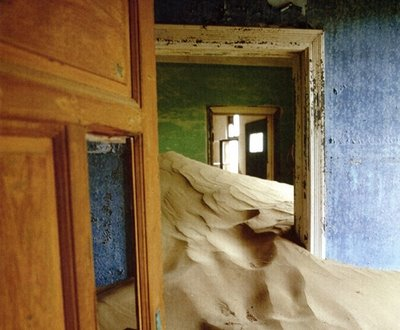
\includegraphics[width=0.5\linewidth]{images/SCP-165-3.jpg}
    \caption*{这张照片,在收容之前拍摄,是通过地表探测无人机拍摄的。}
\end{figure}

这种寄生虫除了最为危险的杀虫剂外,对剩余所有的杀虫剂都有抗药性。如果可以的话,它们会从热源附近撤离并且躲入阴影之中,它们在夜晚时最为活跃,狩猎那些大型的猎物。它们不耐受高温的弱点是最为完美的收容手段。

\hr

\bb{附录 - 获取:}很明显美国政府已经知道SCP-165构成的沙丘有80年的时间了。找到SCP-165的地方现在是一个位于亚利桑那州,菲德立堡之中早被遗忘的闹鬼的德国人移民小镇,在临近金水空军轰炸场的图乐沙漠之中。

这个在菲德立堡中的偏远小镇是在19世纪的某个时候被发现的,并且从1908年开始成为了一个鬼镇。一个途径的骑兵部队报告称所有的居民都消失了,所有的建筑都是空荡荡的。他们想在一个废弃的旅馆之中休整一晚,这样做的结果让他们的7匹马只剩下了骨架,只有4名士兵在半夜逃了出来,他们都说沙子就像洪水一样涌进旅馆之中,这4名士兵再没有被人看见过。

\begin{figure}[H]
    \centering
    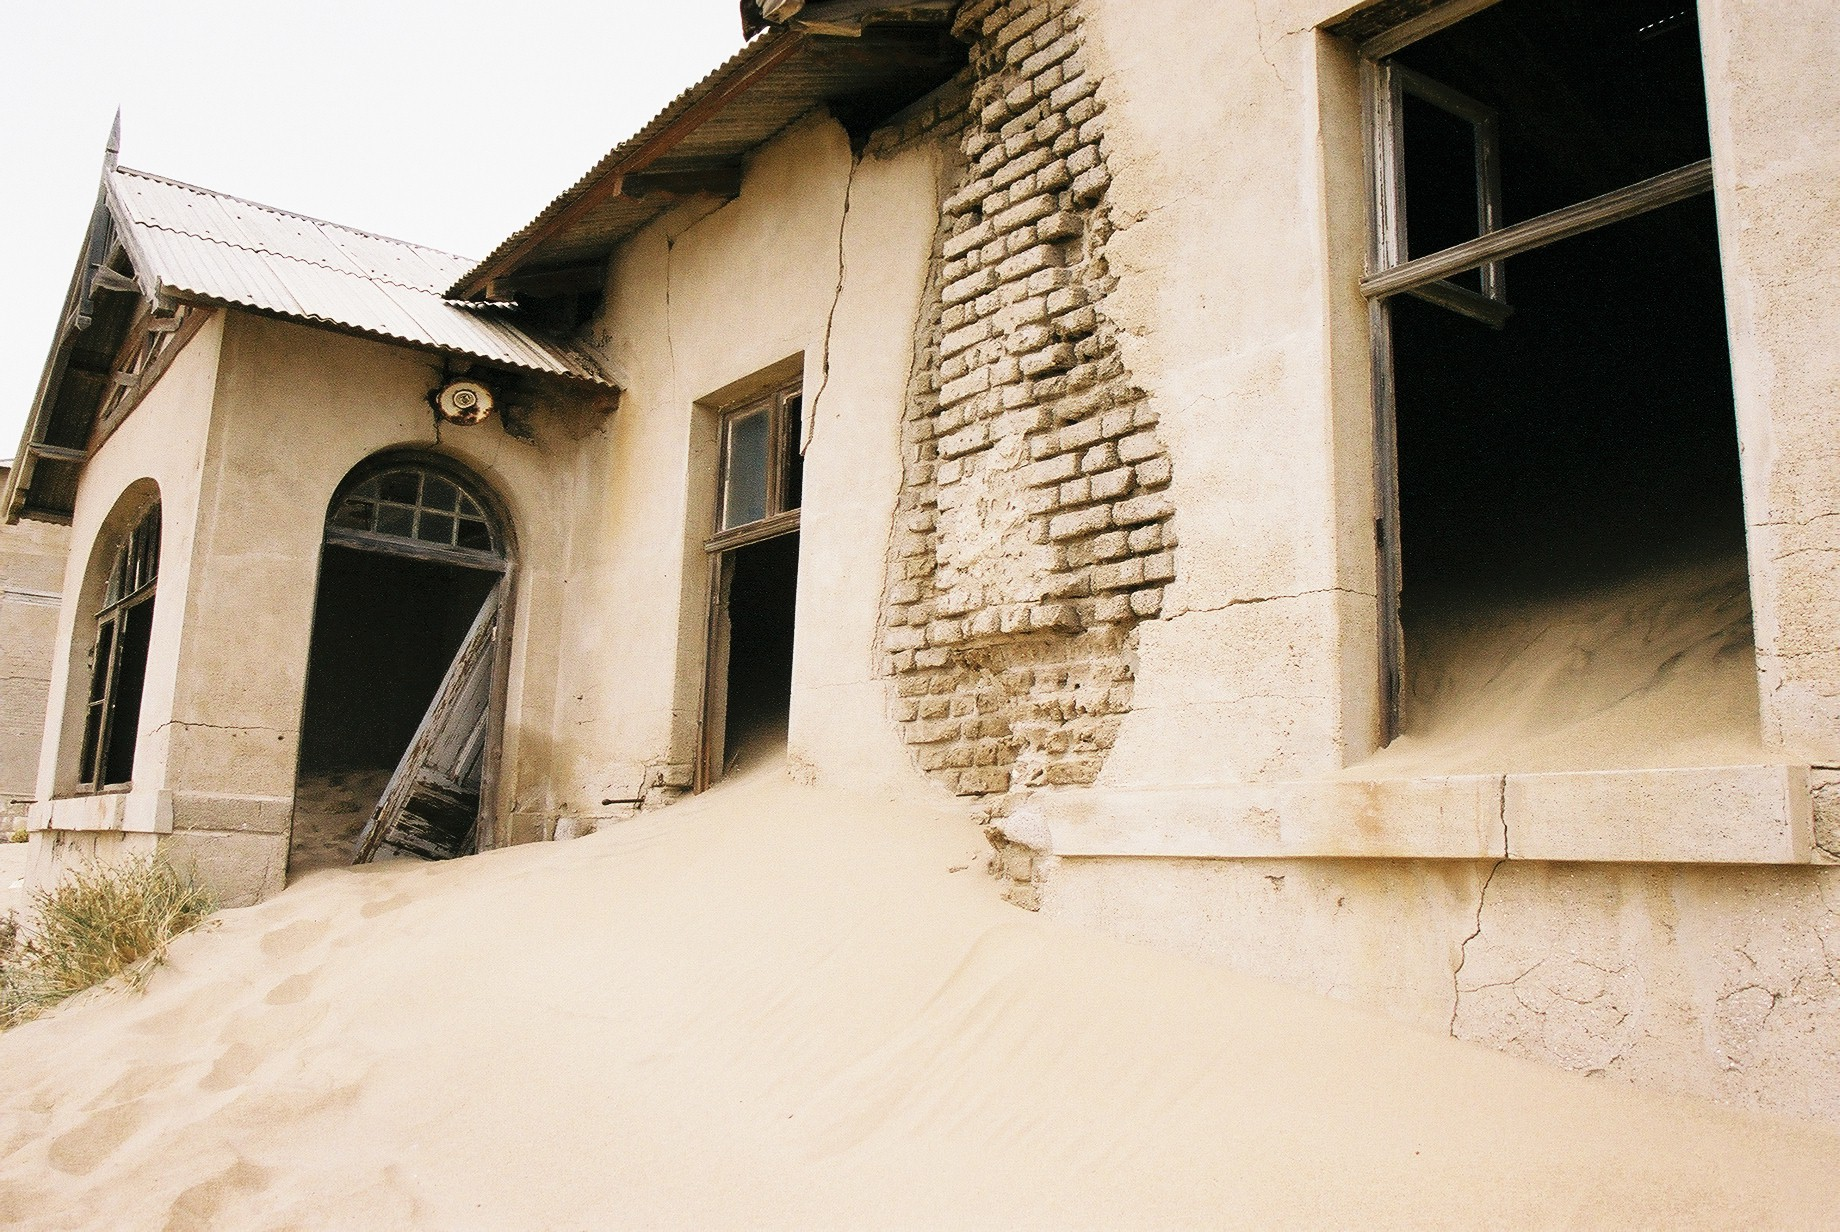
\includegraphics[width=0.5\linewidth]{images/SCP-165-4.jpg}
    \caption*{在亚利桑那州的菲德立堡镇中仍耸立的建筑之中最为完好的一栋,这是SCP-165大形沙丘的家园。}
\end{figure}

在20世纪50年代的晚期,美军试图通过将该区域作为一个轰炸场的方式来根除SCP-165。这个做法成功地减少了SCP-165的数量,但是在20世纪80年代末期,很明显地面的清除和取样对于防止SCP-165的出现是很有必要的。机动特遣队Epsilon-9(又称“噬火者”)被派遣去对SCP-165进行收容和取样。在进入了菲德立堡镇之后,一个上下颠倒的告示牌被发现了,上面写着“Vorsicht vor den kriechenden, hungrigen Sanden”,翻译过来就是“小心蠕动的、贪婪的沙子”。由机动特遣队 \bb{Ɛ}-9携带的火焰喷射器证明能够有效地将SCP-165藏身的沙子玻璃化,并且将它们的数量降低到了一个可以控制的程度。一个大约4t活着的沙丘被收容了并且被转运到14号武装生物收容区域(ABC Area-14),在那里SCP-165得到了监控和收容。

\tred{**从机动特遣队Ɛ-9恢复的图像**}

\tred{关闭}

\begin{longtable}{|l|}
    \hline
    \multicolumn{1}{|l|}{照片 '165-P1';美国,亚利桑那州,弗雷德里克斯堡 - █████ ██,198█}\\
    \hline
    \endhead
    \hline\multicolumn{1}{r}{\small{接下页}}
    \endfoot
    \hline
    \endlastfoot
    \raisebox{-.5\height}{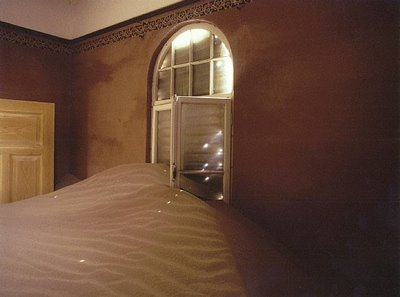
\includegraphics[width=\linewidth]{images/SCP-165-5.jpg}}
\end{longtable}

\begin{longtable}{|l|}
    \hline
    \multicolumn{1}{|l|}{照片 '165-P2';美国,亚利桑那州,弗雷德里克斯堡 - █████ ██,198█}\\
    \hline
    \endhead
    \hline\multicolumn{1}{r}{\small{接下页}}
    \endfoot
    \hline
    \endlastfoot
    \raisebox{-.5\height}{\includegraphics[width=\linewidth]{images/SCP-165-6.jpg}}
\end{longtable}

\begin{longtable}{|l|}
    \hline
    \multicolumn{1}{|l|}{照片 '165-P3';美国,亚利桑那州,弗雷德里克斯堡 - █████ ██,198█}\\
    \hline
    \endhead
    \hline\multicolumn{1}{r}{\small{接下页}}
    \endfoot
    \hline
    \endlastfoot
    \raisebox{-.5\height}{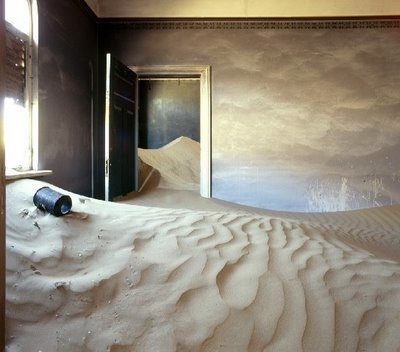
\includegraphics[width=\linewidth]{images/SCP-165-7.jpg}}
\end{longtable}

\tred{关闭}
